\runningheader{SAT Mathematics}{Drill Set 4}{Page \thepage\ of \numpages}

\begingradingrange{sat-drill-04}
\subsection*{SAT Drill 4}



\question[1]
A rectangle has a length that is 15 times its width. The function $y=(15w)(w)$ represents this situation, where $y$ is the area, in square feet, of the rectangle and $y>0$. Which of the following is the best interpretation of $15w$ in this context?
\begin{choices}
  \CorrectChoice The length of the rectangle, in feet
  \choice The area of the rectangle, in square feet
  \choice The difference between the length and the width of the rectangle, in feet
  \choice The width of the rectangle, in feet
\end{choices}

\question[1]
The quadratic function $h$ is defined as shown.
\[
  h(x)=2(x-4)^{2}-32
\]
In the $xy$-plane, the graph of $y=h(x)$ intersects the $x$-axis at the points $(0,0)$ and $(t,0)$, where $t$ is a constant.

What is the value of $t$?
\begin{choices}
  \choice 1
  \choice 2
  \choice 4
  \CorrectChoice 8
\end{choices}

\question[1]
The function $f$ is defined by $f(x)=(-8)(2)^{x}+22$. What is the $y$-intercept of the graph of $y=f(x)$ in the $xy$-plane?
\begin{choices}
  \CorrectChoice $(0,14)$
  \choice $(0,2)$
  \choice $(0,22)$
  \choice $(0,-8)$
\end{choices}


\newpage



\question[1]
The graph shows the height above ground, in meters, of a ball $x$ seconds after the ball was launched upward from a platform. Which statement is the best interpretation of the marked point $(1.0, 4.8)$ in this context?
\begin{center}
  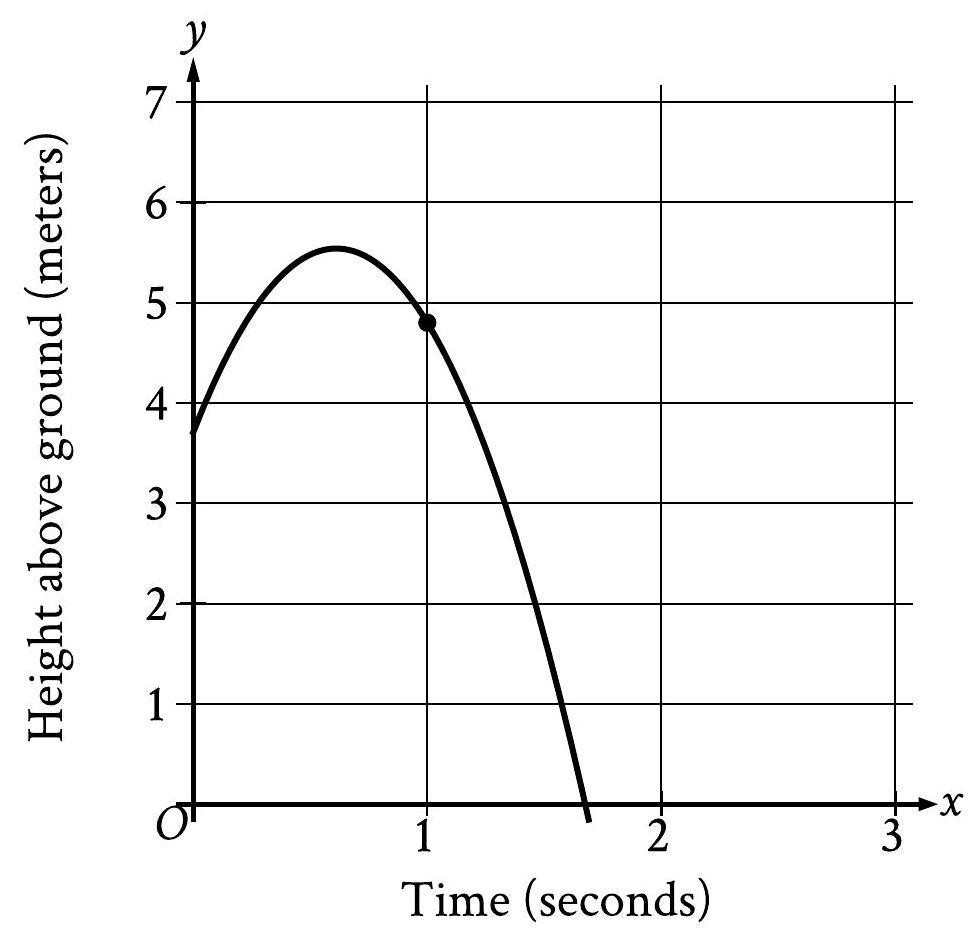
\includegraphics[width=0.70\linewidth]{images/2025_06_15_5ccb8dd1752fe76599e7g-004}
\end{center}
\begin{choices}
  \CorrectChoice 1.0 second after being launched, the ball's height above ground is 4.8 meters.
  \choice 4.8 seconds after being launched, the ball's height above ground is 1.0 meter.
  \choice The ball was launched from an initial height of 1.0 meter with an initial velocity of 4.8 meters per second.
  \choice The ball was launched from an initial height of 4.8 meters with an initial velocity of 1.0 meter per second.
\end{choices}


\question[1]
The first term of a sequence is 9. Each term after the first is 4 times the preceding term. If $w$ represents the $n$th term of the sequence, which equation gives $w$ in terms of $n$?
\begin{choices}
  \choice $w=4\left(9^{n}\right)$
  \choice $w=4\left(9^{n-1}\right)$
  \choice $w=9\left(4^{n}\right)$
  \CorrectChoice $w=9\left(4^{n-1}\right)$
\end{choices}


\newpage


\question[1]
  The given function $f$ models the number of advertisements a company sent to its clients each year, where $x$ represents the number of years since 1997, and $0 \leq x \leq 5$.
  \[
  f(x)=9,000(0.66)^{x}
  \]
  If $y=f(x)$ is graphed in the $xy$-plane, which of the following is the best interpretation of the $y$-intercept of the graph in this context?
\begin{choices}
  \choice The minimum estimated number of advertisements the company sent to its clients during the 5 years was 1,708.
  \choice The minimum estimated number of advertisements the company sent to its clients during the 5 years was 9,000.
  \choice The estimated number of advertisements the company sent to its clients in 1997 was 1,708.
  \CorrectChoice The estimated number of advertisements the company sent to its clients in 1997 was 9,000.
\end{choices}

\question[1]
What is the $y$-intercept of the graph shown?
\begin{center}
  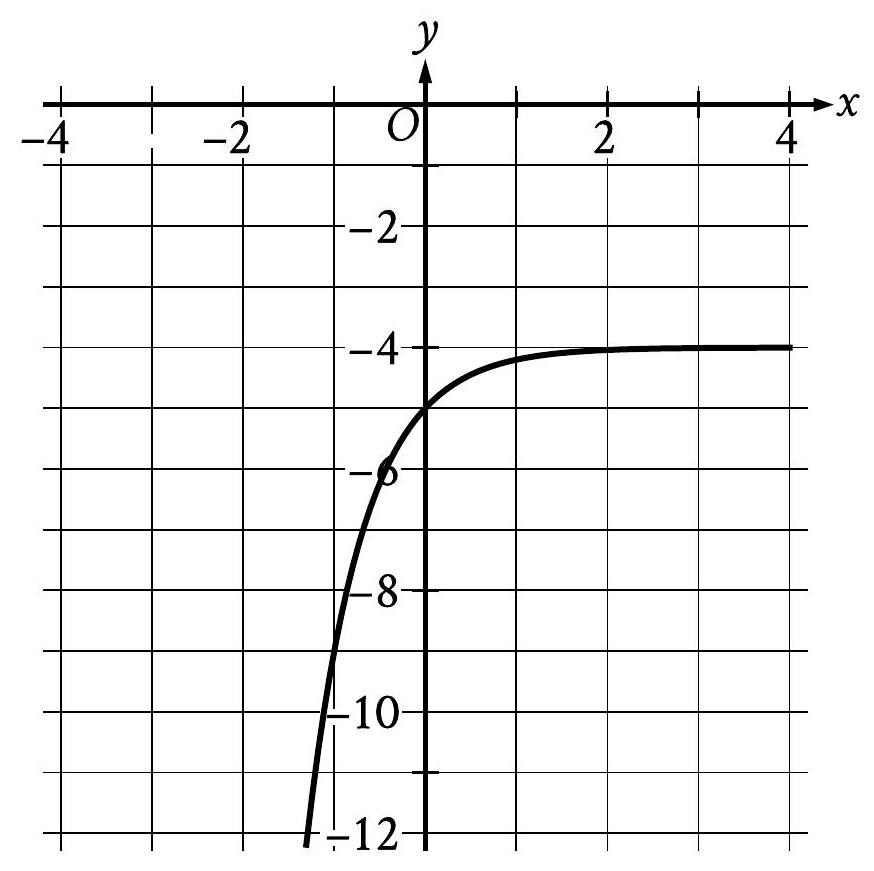
\includegraphics[width=0.70\linewidth]{images/2025_06_15_5ccb8dd1752fe76599e7g-007}
\end{center}
\begin{choices}
  \choice $(-1,-9)$
  \choice $(0,-5)$
  \choice $(0,-4)$
  \choice $(0,0)$
\end{choices}



\newpage


\question[1]
Rosa opened a savings account at a bank. The table below shows the exponential relationship between the time $t$, in years, since Rosa opened the account and the total amount $n$, in dollars, in the account.
  \begin{table}[h!]
  \centering
  \renewcommand{\arraystretch}{1.3}
  \setlength{\tabcolsep}{8pt}
  \caption*{\textbf{Savings Account Balance}}
  \begin{tabular}{|c|c|}
  \hline
  \rowcolor[HTML]{E0E0E0}
  \textbf{Time (years)} & \textbf{Total amount (dollars)} \\
  \hline
  0 & 604.00 \\
  \hline
  1 & 606.42 \\
  \hline
  2 & 608.84 \\
  \hline
  \end{tabular}
  \end{table}
If Rosa made no additional deposits or withdrawals, which of the following equations best represents the relationship between $t$ and $n$?
\begin{choices}
  \CorrectChoice $n=604(1.004)^t$
  \choice $n=604(1.04)^t$
  \choice $n=604(1.004)^{t+1}$
  \choice $n=0.004(604)^t$
\end{choices}

\question[1]
Function $f$ is defined by $f(x)=-a^{x}+b$, where $a$ and $b$ are constants. In the $xy$-plane, the graph of $y=f(x)-12$ has a $y$-intercept at $\left(0,-\frac{75}{7}\right)$. The product of $a$ and $b$ is $\frac{320}{7}$. What is the value of $a$?
\begin{solution}
20
\end{solution}

\newpage


\question[1]
Scientists recorded data about the ocean water levels at a certain location over a period of 6 hours. The graph shown models the data, where $y=0$ represents sea level. Which table gives values of $x$ and their corresponding values of $y$ based on the model?
\begin{center}
  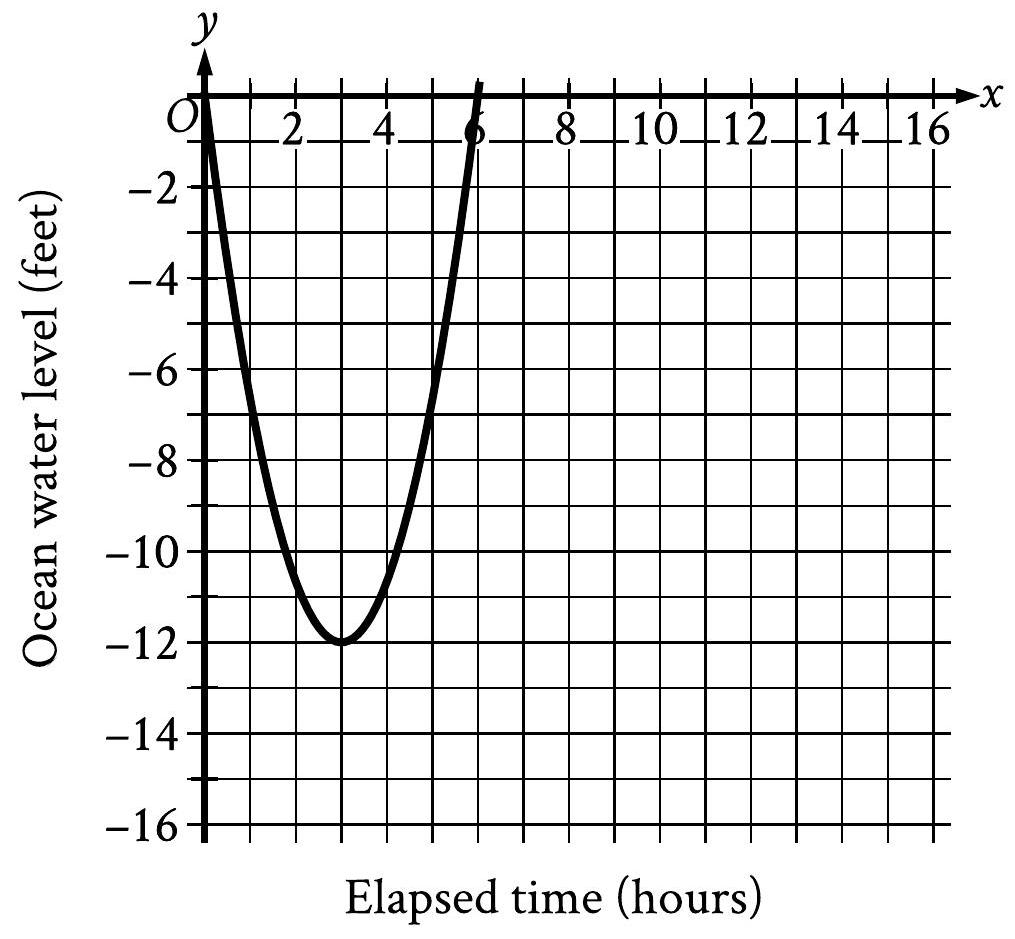
\includegraphics[width=0.90\linewidth]{images/2025_06_15_5ccb8dd1752fe76599e7g-010}
\end{center}
\begin{choices}
  \choice
  \begin{tabular}{|c|c|}
    \hline
    $x$ & $y$ \\
    \hline
    0 & -12 \\
    \hline
    0 & 3 \\
    \hline
    6 & 6 \\
    \hline
  \end{tabular}
  \choice
  \begin{tabular}{|c|c|}
    \hline
    $x$ & $y$ \\
    \hline
    0 & 0 \\
    \hline
    3 & 12 \\
    \hline
    0 & -6 \\
    \hline
  \end{tabular}
  \CorrectChoice
  \begin{tabular}{|c|c|}
    \hline
    $x$ & $y$ \\
    \hline
    0 & 0 \\
    \hline
    3 & -12 \\
    \hline
    6 & 0 \\
    \hline
  \end{tabular}
  \choice
  \begin{tabular}{|c|c|}
    \hline
    $x$ & $y$ \\
    \hline
    0 & 0 \\
    \hline
    12 & 6 \\
    \hline
    -6 & 0 \\
    \hline
  \end{tabular}
\end{choices}

\question[1]
The function $f$ is defined by $f(x)=4+\sqrt{x}$. What is the value of $f(144)$?
\begin{choices}
  \choice 0
  \CorrectChoice 16
  \choice 40
  \choice 76
\end{choices}

\newpage

\question[1]
A rectangular volleyball court has an area of 162 square meters. If the length of the court is twice the width, what is the width of the court, in meters?
\begin{choices}
  \CorrectChoice 9
  \choice 18
  \choice 27
  \choice 54
\end{choices}

\question[1]
A machine launches a softball from ground level. The softball reaches a maximum height of 51.84 meters above the ground at 1.8 seconds and hits the ground at 3.6 seconds. Which equation represents the height above ground $h$, in meters, of the softball $t$ seconds after it is launched?
\begin{choices}
  \choice $h=-t^{2}+3.6$
  \choice $h=-t^{2}+51.84$
  \choice $h=-64(t-2.7)^{2}+51.84$
  \CorrectChoice $h=-16t^{2}+57.6t$
\end{choices}

\question[1]
The function $f$ is defined by $f(x)=a^{x}+b$, where $a$ and $b$ are constants. In the $xy$-plane, the graph of $y=f(x)$ has an $x$-intercept at $(2,0)$ and a $y$-intercept at $(0,-323)$. What is the value of $b$?
\begin{solution}
-324
\end{solution}


\newpage



\question[1]
The function $S$ below models the annual salary, in dollars, of an employee $n$ years after starting a job, where $a$ is a constant.
\[
  S(n)=38,000 a^{n}
\]
If the employee's salary increases by $4\%$ each year, what is the value of $a$?
\begin{choices}
  \choice 0.04
  \choice 0.4
  \CorrectChoice 1.04
  \choice 1.4
\end{choices}

\question[1]
The revenue $f(x)$, in dollars, that a company receives from sales of a product is given by the function below, where $x$ is the unit price, in dollars, of the product.
\[
  f(x)=-500 x^{2}+25\,000 x
\]
The graph of $y=f(x)$ in the $xy$-plane intersects the $x$-axis at 0 and $a$. What does $a$ represent?
\begin{choices}
  \choice The revenue, in dollars, when the unit price of the product is \$0
  \choice The unit price, in dollars, of the product that will result in maximum revenue
  \CorrectChoice The unit price, in dollars, of the product that will result in a revenue of \$0
  \choice The maximum revenue, in dollars, that the company can make
\end{choices}



\newpage



\question[1]
A culture of bacteria is growing at an exponential rate, as shown in the table below.
  \begin{table}[h!]
  \centering
  \renewcommand{\arraystretch}{1.3}
  \setlength{\tabcolsep}{8pt}
  \caption*{\textbf{Growth of a Culture of Bacteria}}
  \begin{tabular}{|c|c|}
  \hline
  \rowcolor[HTML]{E0E0E0}
  \textbf{Day} & \begin{tabular}{c}
  \textbf{Number of bacteria per} \\
  \textbf{milliliter at end of day} \\
  \end{tabular} \\
  \hline
  1 & $2.5 \times 10^{5}$ \\
  \hline
  2 & $5.0 \times 10^{5}$ \\
  \hline
  3 & $1.0 \times 10^{6}$ \\
  \hline
  \end{tabular}
  \end{table}
At this rate, on which day would the number of bacteria per milliliter reach $5.12 \times 10^{8}$?
\begin{choices}
  \choice Day 5
  \choice Day 9
  \choice Day 11
  \CorrectChoice Day 12
\end{choices}

\question[1]
The equation below estimates the global data traffic $D$, in terabytes, for the year that is $t$ years after 2010.
\[
  D=5,640(1.9)^{t}
\]
What is the best interpretation of the number 5,640 in this context?
\begin{choices}
  \choice The estimated amount of increase of data traffic, in terabytes, each year
  \choice The estimated percent increase in the data traffic, in terabytes, each year
  \choice The estimated data traffic, in terabytes, for the year that is $t$ years after 2010
  \CorrectChoice The estimated data traffic, in terabytes, in 2010
\end{choices}



\newpage



\question[1]
In the given quadratic function, $a$ and $c$ are constants. The graph of $y=f(x)$ in the $xy$-plane is a parabola that opens upward and has a vertex at the point $(h, k)$, where $h$ and $k$ are constants.
\[
  f(x)=a x^{2}+4 x+c
\]
If $k<0$ and $f(-9)=f(3)$, which of the following must be true?
\statementbox{
  \begin{enumerate}[label=(\Roman*)]
    \item $c<0$
    \item $a \geq 1$
  \end{enumerate}
}
\begin{choices}
  \choice I only
  \choice II only
  \choice I and II
  \CorrectChoice Neither I nor II
\end{choices}

\question[1]
Which expression is equivalent to $\left(m^{4} q^{4} z^{-1}\right)\left(m q^{5} z^{3}\right)$, where $m$, $q$, and $z$ are positive?
\begin{choices}
  \choice $m^{4} q^{20} z^{-3}$
  \CorrectChoice $m^{5} q^{9} z^{2}$
  \choice $m^{6} q^{8} z^{-1}$
  \choice $m^{20} q^{12} z^{-2}$
\end{choices}

\question[1]
Which of the following is a factor of the polynomial below?
\[
  4 a^{2}+20 a b+25 b^{2}
\]
\begin{choices}
  \choice $a+b$
  \CorrectChoice $2 a+5 b$
  \choice $4 a+5 b$
  \choice $4 a+25 b$
\end{choices}



\newpage



\question[1]
If $p=3 x+4$ and $v=x+5$, which of the following is equivalent to $p v-2 p+v$?
\begin{choices}
  \choice $3 x^{2}+12 x+7$
  \CorrectChoice $3 x^{2}+14 x+17$
  \choice $3 x^{2}+19 x+20$
  \choice $3 x^{2}+26 x+33$
\end{choices}

\question[1]
Which of the following is equivalent to the given expression?
\[
  (x+5)+(2 x-3)
\]
\begin{choices}
  \choice $3 x-2$
  \CorrectChoice $3 x+2$
  \choice $3 x-8$
  \choice $3 x+8$
\end{choices}

\question[1]
Which expression is equivalent to $\frac{8 x(x-7)-3(x-7)}{2 x-14}$, where $x>7$?
\begin{choices}
  \choice $\frac{x-7}{5}$
  \CorrectChoice $\frac{8 x-3}{2}$
  \choice $\frac{8 x^{2}-3 x-14}{2 x-14}$
  \choice $\frac{8 x^{2}-3 x-77}{2 x-14}$
\end{choices}

\question[1]
Which of the following is equivalent to the expression $x^{4}-x^{2}-6$?
\begin{choices}
  \choice $\left(x^{2}+1\right)\left(x^{2}-6\right)$
  \CorrectChoice $\left(x^{2}+2\right)\left(x^{2}-3\right)$
  \choice $\left(x^{2}+3\right)\left(x^{2}-2\right)$
  \choice $\left(x^{2}+6\right)\left(x^{2}-1\right)$
\end{choices}

\question[1]
Which of the following is equivalent to the expression below?
\[
  (2 x+5)^{2}-(x-2)+2(x+3)
\]
\begin{choices}
  \CorrectChoice $4 x^{2}+21 x+33$
  \choice $4 x^{2}+21 x+29$
  \choice $4 x^{2}+x+29$
  \choice $4 x^{2}+x+33$
\end{choices}



\question[1]
The equation below is true for all $x$, where $a$ and $b$ are constants.
\[
  (a x+3)\left(5 x^{2}-b x+4\right)=20 x^{3}-9 x^{2}-2 x+12
\]
What is the value of $a b$?
\begin{choices}
  \choice 18
  \choice 20
  \CorrectChoice 24
  \choice 40
\end{choices}

\question[1]
Which of the following expressions is equivalent to $x^{2}-5$?
\begin{choices}
  \choice $(x+\sqrt{5})^{2}$
  \choice $(x-\sqrt{5})^{2}$
  \CorrectChoice $(x+\sqrt{5})(x-\sqrt{5})$
  \choice $(x+5)(x-1)$
\end{choices}



\newpage




\question[1]
Which of the following expressions is(are) a factor of $3 x^{2}+20 x-63$?
\statementbox{
  \begin{enumerate}[label=(\Roman*)]
    \item $x-9$
    \item $3 x-7$
  \end{enumerate}
}
\begin{choices}
  \choice I only
  \CorrectChoice II only
  \choice I and II
  \choice Neither I nor II
\end{choices}

\question[1]
If $\frac{\sqrt{x^{5}}}{\sqrt[3]{x^{4}}}=x^{\frac{a}{b}}$ for all positive values of $x$, what is the value of $\frac{a}{b}$?
\begin{solutionorbox}
We have $\sqrt{x^{5}}=x^{5/2}$, $\sqrt[3]{x^{4}}=x^{4/3}$, so the quotient is $x^{5/2-4/3}=x^{7/6}$ and $\frac{a}{b}=\frac{7}{6}$.
\end{solutionorbox}

\question[1]
The expression $90 y^{5}-54 y^{4}$ is equivalent to $r y^{4}(15 y-9)$, where $r$ is a constant. What is the value of $r$?
\begin{solutionorbox}
Factor: $90 y^{5}-54 y^{4}=6 y^{4}(15 y-9)$, so $r=6$.
\end{solutionorbox}



\newpage



\question[1]
The equation below is true for all $x>2$, where $r$ and $t$ are positive constants.
\[
  \frac{2}{x-2}+\frac{3}{x+5}=\frac{r x+t}{(x-2)(x+5)}
\]
What is the value of $r t$?
\begin{choices}
  \choice -20
  \choice 15
  \CorrectChoice 20
  \choice 60
\end{choices}

\question[1]
Which of the following is an equivalent form of $(1.5 x-2.4)^{2}-\left(5.2 x^{2}-6.4\right)$?
\begin{choices}
  \choice $-2.2 x^{2}+1.6$
  \choice $-2.2 x^{2}+11.2$
  \CorrectChoice $-2.95 x^{2}-7.2 x+12.16$
  \choice $-2.95 x^{2}-7.2 x+0.64$
\end{choices}

\question[1]
For what value of $x$ is the given expression equivalent to $(70 n)^{30 x}$, where $n>1$?
\[
  \sqrt[5]{70 n}(\sqrt[6]{70 n})^{2}
\]
\begin{solutionorbox}
The expression equals 
$$(70 n)^{1/5}(70 n)^{1/3}=(70 n)^{8/15}$$
so 
$$30 x=\frac{8}{15}$$
and
$$x=\frac{4}{225}$$
\end{solutionorbox}



\newpage



\question[1]
A system of equations consists of a quadratic equation and a linear equation. The equations in this system are graphed in the $xy$-plane below.

\begin{center}
  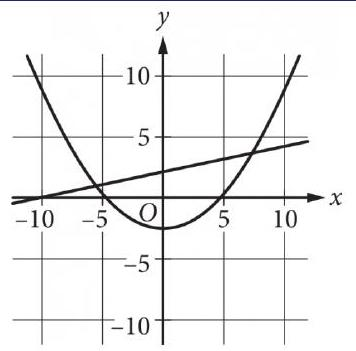
\includegraphics[width=0.90\linewidth]{images/2025_06_15_6ec744ffc48635e98821g-01}
\end{center}
How many solutions does this system have?
\begin{choices}
  \choice 0
  \choice 1
  \CorrectChoice 2
  \choice 3
\end{choices}

\question[1]
Which of the following inequalities is equivalent to the inequality above?
\[
  6 x-9 y>12
\]
\begin{choices}
  \choice $x-y>2$
  \CorrectChoice $2 x-3 y>4$
  \choice $3 x-2 y>4$
  \choice $3 y-2 x>2$
\end{choices}



\newpage



\question[1]
If $(x, y)$ is a solution to the system of equations above, which of the following could be the value of $x$?
\[
  \begin{aligned}
  & y=x+1 \\
  & y=x^{2}+x
  \end{aligned}
\]
\begin{choices}
  \CorrectChoice -1
  \choice 0
  \choice 2
  \choice 3
\end{choices}

\question[1]
What values satisfy the equation above?
\[
  x^{2}-x-1=0
\]
\begin{choices}
  \choice $x=1$ and $x=2$
  \choice $x=-\frac{1}{2}$ and $x=\frac{3}{2}$
  \CorrectChoice $x=\frac{1+\sqrt{5}}{2}$ and $x=\frac{1-\sqrt{5}}{2}$
  \choice $x=\frac{-1+\sqrt{5}}{2}$ and $x=\frac{-1-\sqrt{5}}{2}$
\end{choices}

\question[1]
The graphs of the given equations intersect at the point $(x, y)$ in the $xy$-plane.
\[
  \begin{gathered}
  x=49 \\
  y=\sqrt{x}+9
  \end{gathered}
\]
What is the value of $y$?
\begin{choices}
  \CorrectChoice 16
  \choice 40
  \choice 81
  \choice 130
\end{choices}



\newpage



\question[1]
What is the positive solution to the given equation?
\[
  2|4-x|+3|4-x|=25
\]
\begin{solutionorbox}
  $9$
\end{solutionorbox}

\question[1]
One solution to the given equation can be written as $1+\sqrt{k}$, where $k$ is a constant.
\[
  x^{2}-2 x-9=0
\]
What is the value of $k$?
\begin{choices}
  \choice 8
  \CorrectChoice 10
  \choice 20
  \choice 40
\end{choices}

\question[1]
In the $xy$-plane, a line with equation $2 y=4.5$ intersects a parabola at exactly one point. If the parabola has equation $y=-4 x^{2}+b x$, where $b$ is a positive constant, what is the value of $b$?
\begin{solutionorbox}
  $6$
\end{solutionorbox}



\newpage



\question[1]
The graph of a system of a linear equation and a nonlinear equation is shown.

\begin{center}
  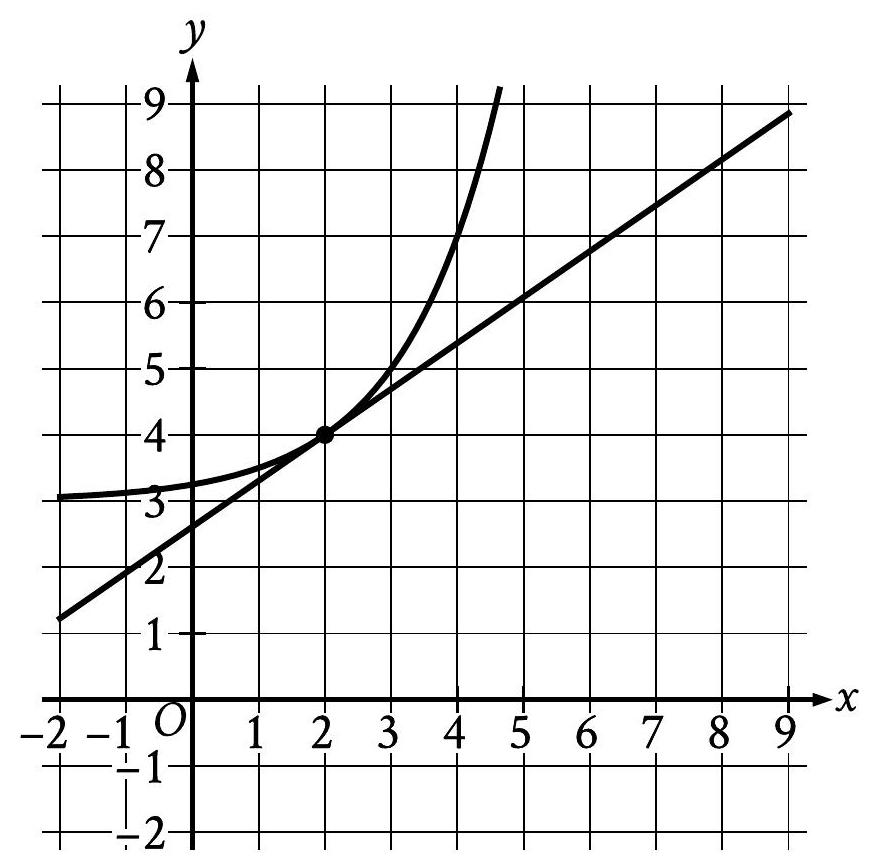
\includegraphics[width=0.90\linewidth]{images/2025_06_15_6ec744ffc48635e98821g-17}
\end{center}
What is the solution $(x, y)$ to this system?
\begin{choices}
  \choice $(0,0)$
  \choice $(0,2)$
  \CorrectChoice $(2,4)$
  \choice $(4,0)$
\end{choices}

\question[1]
What is the product of the solutions to the given equation?
\[
  (x-4)(x+2)(x-1)=0
\]
\begin{choices}
  \choice 8
  \choice 3
  \choice -3
  \CorrectChoice -8
\end{choices}



\newpage



\question[1]
What is the solution to the equation above?
\[
  \frac{2(x+1)}{x+5}=1-\frac{1}{x+5}
\]
\begin{choices}
  \choice 0
  \CorrectChoice 2
  \choice 3
  \choice 5
\end{choices}

\question[1]
What is the smallest solution to the given equation?
\[
  \sqrt{(x-2)^{2}}=\sqrt{3 x+34}
\]
\begin{solutionorbox}
  $-3$
\end{solutionorbox}

\endgradingrange{sat-drill-04}
